\documentclass[12pt,letterpaper]{article}
\usepackage[spanish]{babel}
\usepackage[utf8]{inputenc}    %Uso de tildes si desarrolla en Linux
%\usepackage[latin1]{inputenc}   %Uso de tildes si desarrolla en Windows
\usepackage{setspace} %define comandos \singlespacing, \onehalfspacing, \doublespacing
\usepackage[left=1.5cm, right=1.5cm, top=1.5cm, bottom=1.5cm]{geometry}
\usepackage{graphicx}
\usepackage{amssymb}
\usepackage{epsfig}
\usepackage{url}
\usepackage[pdftex,
	    breaklinks=true,
	    linktocpage=true,
	    pdfborder={0 0 0},
	    pdftoolbar=true,
	    colorlinks=true,
	    linkcolor=blue,
	    citecolor=blue,
	    filecolor=blue,
	    urlcolor=blue]{hyperref}

\begin{document}


{\begin{tabular}{ccc}
  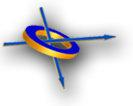
\includegraphics[width=15mm]{ECCI.jpg}& 
  \parbox{6in}{ \centering 
                  \small \textbf{Universidad de Costa Rica\\
                      Escuela de Ciencias de la Computación e Informática\\
                      CI-0119 Proyecto Integrador de Lenguaje Ensamblador y Arquitectura\\
                      I ciclo de 2019}\\
                     \hrulefill
                 }  & 
  
\includegraphics[width=15mm]{UCR.jpg}\\
 \end{tabular}
}

{\centering {\Large \textbf{Proyecto 2\\}} }

\section*{Objetivo general}
\begin{itemize}
 \item Construir un sistema que evalúa funciones vectoriales por medio de un módulo de kernel, simulando un dispositivo matemático especializado, un manejador de dispositivo (device driver) para interactuar con el módulo de kernel y una aplicación de software para definir y representar gráficamente las funciones. El sistema a construir debe utilizar las funciones de procesamiento vectorial disponibles en los microprocesadores modernos en el nivel del lenguaje ensamblador.
\end{itemize}

\section*{Objetivos específicos}
\begin{itemize}
 \item Diseñar e implementar un módulo de kernel, en el sistema operativo Linux, que llamaremos \textit{VFunction}, el cual se especializará en la ejecución de funciones matemáticas para cálculo y representación de funciones evaluadas en vectores con datos multidimensionales.
 \item Diseñar e implementar un device driver \textit{VFunctionDev} para habilitar la interacción de aplicaciones de software con el dispositivo \textit{VFunction}, a través de llamados al sistema operativo.
 \item Diseñar e implementar una aplicación de software que permita evaluar los módulos \textit{VFunction} y \textit{VFunctionDev}, a través de la interacción de funciones en lenguaje C/C++ y ensamblador.
\end{itemize}

\section*{Descripción del sistema para cálculo de funciones vectoriales}

En este proyecto su equipo de trabajo debe construir un sistema para calcular y representar funciones vectoriales que esté compuesto por 3 elementos:
\begin{enumerate}

\item \textit{Aplicación de software}: una aplicación de software para graficar funciones vectoriales, escrita en los lenguajes de alto nivel C o C++, que permita representar visualmente coordenadas de funciones vectoriales generadas por el módulo VFunction. El sitio web https://www.desmos.com/calculator presenta una aplicación de software interesante, para construir funciones vectoriales de 2 dimensiones, y que puede utilizar para familiarizarse con este tipo de funciones.

\item \textit{VFunctionDev}: un device driver que será usado como mecanismo para interpretar (parsing) la expresión matemática para la función dada por el usuario desde la aplicación de software, analizarla, y darle una representación apropiada para ser procesada por el módulo \textit{VFunction}, como por ejemplo descomponer la función vectorial en sus operandos, operadores, rango de evaluación, entre otros, para su correcta ejecución a través de \textit{VFunction}. 

\item \textit{VFunction}: un módulo de kernel en Linux especializado en el cálculo de funciones vectoriales en 2 y 3 dimensiones. El módulo debe ser programado utilizando las funciones especializadas y de procesamiento vectorial del lenguaje ensamblador y disponibles en los microprocesadores modernos. \textit{VFunction} recibe como entrada la especificación de la función vectorial, incluyendo todos los parámetros apropiados para evaluarla, como por ejemplo la especificación de la función a calcular, su fórmula, rangos de valores, entre otros, y genera un vector de valores que permite graficarla de buena forma por medio de la aplicación de software. Es decir, el módulo calcula los valores de la función pero \underline{no} grafica o despliega datos en una pantalla o en ningún otro dispositivo de salida. Las tareas de despliegue serán responsabilidad de la aplicación de alto nivel. El formato estructurado de los parámetros generados por \textit{VFunctionDev} y que serán enviados a \textit{VFunction} es parte de las tareas de diseño del proyecto.

\end{enumerate} 
En la figura siguiente se muestra la interacción entre la aplicación de software, el device driver \textit{VFunctionDev}, y el módulo \textit{VFunction}.

\begin{verbatim}
        ------------                ---------------                -------------
        |          | llamado S.O.   |     S.O.    | llamado entre  |           |
        |Aplicación| (syscall)      | ----------- | módulos        |Dispositivo|
        |   de     |<-------------->| |VFunction| |<-------------->| VFunction |
        |software  | Parámetros en  | |   Dev   | | Parámetros en  |           |
        |          | formato texto  | ----------- | formato        |           |
        ------------                --------------- estructurado   -------------
        interactúa                  recibe solicitud a              ejecuta el 
          con el                    través de syscall,              cálculo de 
         usuario                    analiza la entrada              la función
                                    invoca a VFunction
 \end{verbatim}

\section*{Requerimientos de la aplicación de software}
La aplicación de software tiene los siguientes requerimientos: 
\begin{itemize}                                                                                                                                                                                                                                                                                                                                                                                                                                                                                                                                                            \item \textit{Entrada de datos}: recibe del usuario final la definición de una función vectorial, así como los parámetros (rangos y otros valores) requeridos para evaluarla y graficarla. Los datos de entrada serán ingresados por medio de una o varias hileras de texto, intentando mantener un formato simple en la entrada de datos para el usuario. Las hileras con la especificación de la función deben ser enviadas al device driver \textit{VFunctionDev} para validación, análisis (parsing) y posterior envío al módulo \textit{VFunction} para evaluación de la función. La aplicación de software no debe tener vulnerabilidades de buffer overflow en la captura de datos y en la mayor medida posible tampoco en la interacción entre los componentes del sistema a desarrollar. Más adelante se describe el nivel de complejidad que pueden tener las expresiones para las funciones vectoriales y para sus rangos de evaluación.
\item \textit{Interacción con el S.O.}: invoca al device driver \textit{VFunctionDev} para que éste haga su trabajo de analizar y estructurar las hileras capturadas y genere una invocación al módulo \textit{VFunction}, para que calcule las coordenadas de la función vectorial y las entregue de vuelta a la aplicación. 
\item \textit{Graficar la función}: despliega en pantalla la función vectorial en 2 ó 3 dimensiones, según corresponda, por medio de alguna biblioteca de gráficos en C/C++ como OpenGL o Qt.                                                                                                                                                                                                                                                                                                                                                                                                                                                                                                                                                                 

\end{itemize}

\section*{Requerimientos del device driver \textit{VFunctionDev}}
El device driver tiene los siguientes requerimientos:
\begin{itemize}

\item \textit{Comunicación con la aplicación}: la comunicación entre la aplicación de software y el device driver \textit{VFunctionDev} debe realizarse por medio de llamados estándar al sistema operativo (system calls) utilizando las funciones de la biblioteca estándar. El driver \textit{VFunctionDev} requiere enviar y recibir información entre la aplicación de usuario y el dispositivo, por lo cual debe seleccionar apropiadamente la interfaz requerida. 
\item \textit{Comunicación con el módulo VFunction}: la comunicación entre el device driver \textit{VFunctionDev} y el módulo \textit{VFunction} debe realizarse usando mecanismos estándar provistos por el sistema operativo, por medio de llamados entre módulos de kernel. 
El device driver es la pieza de software que recibe la función a graficar, desde la aplicación de software especificada por medio de una o varias hileras de texto, la valida, la interpreta y la representa en un formato apropiado para que el módulo de kernel \textit{VFunction} realice los cálculos de las coordenadas vectoriales que serán usadas para su representación gráfica. 
\item \textit{Interpretación de las funciones y rangos de evaluación}: el device driver debe tomar las hileras de texto capturadas en la aplicación de software, las cuales contienen la definición de la función a evaluar, así como la definición de los rangos de valores en que debe ser evaluada, y debe estructurar la información recibida de forma tal que el módulo \textit{VFunction} solamente requiera hacer un trabajo menor de identificación de los cálculos que debe realizar, para obtener las coordenadas de puntos a graficar. En la sección \textbf{Complejidad de las expresiones para funciones vectoriales y rangos de evaluación}, más adelante, se describen las consideraciones específicas y niveles de complejidad de las funciones que pueden ser evaluadas y aspectos del formato de los rangos de valores para la evaluación.
\item \textit{Módulo de kernel}: el device driver debe ser desarrollado como un módulo de kernel para el sistema operativo Linux. Utilice una versión reciente de Linux y que sea compatible, en su ejecución, con el módulo de kernel del dispositivo \textit{VFunction}.
\item \textit{Programación del módulo con el device driver}: la programación de la estructura general del device driver puede estar escrita en lenguaje C, pero las operaciones de análisis e interpretación de las hileras, conteniendo expresiones de funciones y rangos de evaluación de las mismas, deben escribirse en lenguaje ensamblador.
\end{itemize}

 
\section*{Requerimientos del módulo \textit{VFunction}}
El módulo \textit{VFunction} tiene los siguientes requerimientos:
\begin{itemize}
\item \textit{Comunicación con el device driver}: el módulo de kernel del dispositivo debe contar con una interfaz y las previsiones necesarias para comunicarse solamente con el device driver y no puede interactuar directamente con las aplicaciones de software.
\item \textit{Procesamiento de funciones vectoriales}: el módulo \textit{VFunction} debe ser capaz de tomar la especificación de una función vectorial y los rangos en que debe ser evaluada y producir un vector de coordenadas multidimensionales (2D o 3D) que serán devueltos a la aplicación de software como resultado de la operación, a través del device driver.
\item \textit{Cálculo de coordenadas de la función}: la evaluación de la funciones en los rangos de valores indicados debe hacerse en lenguaje ensamblador. La programación de los cálculos debe utilizar de la mejor forma posible las tecnologías de apoyo a procesamiento paralelo y funciones matemáticas incluídas en los procesadores Intel modernos, dentro de las cuales se deben valorar SSE, SSE2, SSE3, SSSE3, SSE4, AVX, AVX2 y AVX512. De forma especial considere y seleccione, durante la etapa de diseño, las instrucciones de tipo SIMD (Single Instruction Multiple Data) que permiten ejecutar operaciones en paralelo sobre grupos de datos.
\item \textit{Módulo de kernel}: el módulo \textit{VFunction} debe estar implementado como un módulo de kernel para el sistema operativo Linux de una versión reciente. La programación de la estructura del módulo de kernel puede estar escrita en lenguaje C, según se documenta extensivamente en la literatura relacionada con el desarrollo de módulos de kernel para Linux.
\end{itemize}

\section*{Complejidad de las expresiones para funciones vectoriales y rangos de evaluación}
Con el fin de mantener el nivel de complejidad del proyecto en un nivel apropiado, en esta sección se define el formato de las expresiones aritméticas que debe ser usado para especificar las funciones vectoriales, según se detalla a continuación:
\begin{itemize}
\item Funciones vectoriales pueden ser de 2 ó 3 dimensiones.
\item Los componentes de las funciones pueden estar en término de 1 o 2 variables. La primera variable siempre se llama \textit{x} y la segunda variables siempre se llama \textit{y}
\item Las expresiones matemáticas para las funciones que conforman cada función vectorial son sumas de productos que contienen hasta 3 términos en suma/resta y hasta 3 elementos en multiplicación/división por cada término.
\item Elementos válidos en cada término pueden ser: las variables de la función, valores constantes, funciones matemáticas predefinidas en el microprocesador y aplicadas a las variables de la función, debe soportar al menos 3 funciones predefinidas (por ejemplo, sin(t), cos(t), etc.).
Los siguientes son ejemplos de funciones válidas para expresar una de las dimensiones de una función vectorial:
\begin{verbatim}
    f(x) = 3*x*x + x - 2       (función con 3 términos (3*x*x, x, 2). El 
          ------- --- ---       primer término tiene 3 elementos (3, x, x)).
          
Otros ejemplos de funciones son:
    f(x) = sin(x) * 4          (función de un término con 2 elementos)
    f(x, y) = cos(x) + sin(y)  (función de dos términos con un elemento cada uno)
    
\end{verbatim} 

Una función vectorial estaría compuesta por dos o tres funciones de una dimensión, por ejemplo, el siguientes es un ejemplo de una función vectorial de 3 dimensiones y de una variable:
\begin{verbatim}
         cos(x), 4+ln(x), sqrt(x)
\end{verbatim}
Note que expresiones como sqrt(x+1) en donde la complejidad de la expresión es mayor, por cuanto el término x + 1 está anidado en la expresión sqrt(), no son requeridos pero podrían ser opcionalmente implementados si el tiempo lo permite y el grupo de proyecto lo acuerda.

En relación con los rangos de evaluación de las funciones, se tienen las siguientes consideraciones:
\item Se pueden especificar hasta 3 rangos de valores para evaluar la función vectorial, indicados como intervalos cerrados de números reales, la implementación de intervalos abiertos es opcional.
\item Los rangos de evaluación deben ir acompañados de un valor de incremento, que será usado para seleccionar los valores en el rango que serán evaluados y graficados.
\end{itemize}
El siguiente es un ejemplo de valores para evaluar una función vectorial de una variable, por medio de 3 rangos y con un incremento de 0.01 entre los valores calculados.
\begin{verbatim}
 [0 1] [5 7] [10 15] 0.01
\end{verbatim} 

\section*{Manejo de errores en la aplicación y en los módulos}

El manejo de condiciones de error es un aspecto esencial en todo sistema de software y en particular en sistemas de software donde participa el sistema operativo de forma directa. Dado este contexto, es parte de los requerimientos generales de su proyecto las siguientes consideraciones para manejo de errores:
\begin{itemize}
 \item El módulo \textit{VFunction} debe detectar errores de indefinición en el cálculo de las funciones y reportarlos al device driver \textit{VFunctionDev}. Cuando se detecta algún error, el módulo cancelará los cálculos solicitados y devolverá un código de error apropiado a \textit{VFunctionDev}, por medio de los mecanismos estándar definidos por el sistema operativo.
 \item El device driver \textit{VFunctionDev} debe detectar errores de sintaxis en las hileras que contienen la especificación de las funciones y los rangos de evaluación.  Cuando se detecta algún error, el device driver no invocará al módulo \textit{VFunction} y devolverá un código de error a la aplicación de software, por medio de los mecanismos estándar definidos por el sistema operativo.
 \item La aplicación de software debe realizar controles de error razonables para sus tareas propias, y mostrar mensajes apropiados para los códigos de error devueltos por los módulos de kernel.
\end{itemize}


\section*{Actividades a realizar}
\begin{itemize}
 \item Establecer y escribir el plan de trabajo.
 \item Definir y escribir el diseño integral de todos los componentes del sistema gráfico.
 \item Construir y documentar la solución de software propuesta.
 \item Ejecutar la evaluación funcional de \textit{VFunction} y \textit{VFunctionDev} por medio de la aplicación de software.
 \item Realizar informes de avance semanales durante todo el desarrollo del proyecto.
\end{itemize}

\section*{Metodología, cronograma y evaluación}
Se trabajará en grupos según se establece en el programa del curso. Durante las lecciones el profesor dará guías generales sobre cómo construir el plan de trabajo, el diseño y la implementación del proyecto. Cada grupo acordará una estrategia de trabajo, establecerá un diseño, lo implementará, lo documentará y lo defenderá en clase. 

\textbf{Nota importante}: la programación de módulos de kernel y devices drivers en Linux requiere que el desarrollador tenga permisos de usuario root en el computador donde se carguen y ejecuten los módulos, por lo cual esta es una consideración a tener presente durante el desarrollo del proyecto. Una solución a este situación puede ser trabajar en una máquina virtual, en cuyo caso también deben considerarse la disponibilidad de las extensiones de multimedios para ensamblador en la versión de la máquina virtual utilizada.

El proyecto se entregará por partes, como se indica a continuación.
\begin{itemize}
 \item Inicio del proyecto: entrega del enunciado.
       Fecha de entrega: 23 de mayo.
 \item Primer entregable: un documento con el plan de trabajo.
       Fecha de entrega: 6 de junio (2 semanas). Valor 15\%.
 \item Segundo entregable: un documento con el diseño detallado del sistema.
       Fecha de entrega: 20 de junio (2 semanas). Valor 30\%.
 \item Tercer entregable: implementación del sistema gráfico y su documentación final. 
       Fecha de entrega 11 de julio (3 semanas). Valor 30\%.
 \item Cuarto entregable: Presentación y defensa del proyecto. 
       Fecha: semana del 15 al 19 de julio (1 semana). Valor 10\%.
 \item Quinto entregable: Informes de avance cada semana. 
       Fecha: cada día de clase. Valor 15\%.
\end{itemize}

\section*{Estructura del documento con el plan de trabajo}

 \begin{itemize}
 \item Descripción general: que describa las características principales del sistema a construir.
 \item Marco teórico: que contemple los fundamentos de los principales componentes del sistema gráfico.
 \item Diseño preliminar: contiene una primera versión, de muy alto nivel, con la especificación técnica del sistema a desarrollar. Incluye algunas decisiones y consideraciones que guían las siguientes etapas del diseño. También se recomienda incluir un índice preliminar del documento de diseño.
 \item Cronograma de actividades: contiene la lista detallada de actividades a realizar, indicando una descripción suficientemente clara del alcance de cada una y las fechas propuestas de ejecución, considerando como marco de referencia las fechas de entrega del enunciado del proyecto. Planifique entregas semanales, con al menos un punto de revisión adicional a lo interno de su grupo de trabajo durante la semana.
 \item Organización/distribución de tareas: describe la distribución de responsabilidades y trabajo entre los miembros del equipo y debe integrarse con el cronograma de actividades.  
 \item Referencias bibliográficas usadas para la elaboración del plan y que serán usadas para la elaboración del proyecto.
 \end{itemize}

\section*{Estructura de los informes de avance}

 \begin{enumerate}
 \item Encabezado con la información de los miembros del equipo, la fecha del informe y el periodo de tiempo que se considera en el informe.
 \item Una tabla con lista de actividades que estaban programadas para el periodo de tiempo reportado, indicando las que fueron ejecutadas, las que no fueron ejecutadas y un espacio para comentarios, principalmente para justificaciones en casos especiales.
 \item Tareas realizadas por cada miembro del equipo.
 \item Acuerdos relevantes, sean técnicos o logísticos, tomados durante la semana en relación con el desarrollo del proyecto.
 \end{enumerate}

\end{document}
%------------------------------------------------------------
